\begin{tikzpicture}[
    >=Latex,
    node distance=1.6cm and 0.7cm,
    every node/.style={font=\small},
    stage/.style={
        rectangle, rounded corners=3pt, draw, thick,
        fill=blue!8, minimum width=2.7cm, minimum height=2.0cm,
        align=center, inner sep=4pt,
    },
    flow/.style={->, very thick, blue!50!black},
    flowlabel/.style={font=\scriptsize, gray!70!black, fill=white,
                      inner sep=2pt, align=center},
    iolabel/.style={font=\scriptsize\bfseries, gray!70!black,
                    align=center},
]
    % =========================================================
    % Reihe 1: Stufen 1 bis 3
    % =========================================================
    \node[stage] (s1) {%
        \textbf{1}\\[-2pt]
        \scriptsize Schichtpositionen\\[2pt]
        \begin{tikzpicture}[baseline]
            \draw[gray!50] (0, 0) rectangle (0.6, 0.45);
            \foreach \y in {0.075, 0.225, 0.375} {
                \draw[blue!70!black, thin] (-0.05, \y) -- (0.65, \y);
            }
        \end{tikzpicture}
    };

    \node[stage, right=of s1] (s2) {%
        \textbf{2}\\[-2pt]
        \scriptsize Schnitt\\[2pt]
        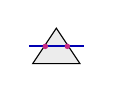
\begin{tikzpicture}[baseline]
            \fill[gray!15] (0, 0) -- (0.6, 0) -- (0.3, 0.45) -- cycle;
            \draw (0, 0) -- (0.6, 0) -- (0.3, 0.45) -- cycle;
            \draw[blue!70!black, thick] (-0.05, 0.22) -- (0.65, 0.22);
            \fill[magenta!80!black] (0.16, 0.22) circle (1pt);
            \fill[magenta!80!black] (0.44, 0.22) circle (1pt);
        \end{tikzpicture}
    };

    \node[stage, right=of s2] (s3) {%
        \textbf{3}\\[-2pt]
        \scriptsize Verkettung\\[2pt]
        
\begin{tikzpicture}[baseline]
            \draw[magenta!80!black, very thick]
                (0.08, 0.10) -- (0.22, 0.05) -- (0.42, 0.05) --
                (0.56, 0.15) -- (0.56, 0.30) -- (0.42, 0.40) --
                (0.22, 0.40) -- (0.08, 0.30) -- cycle;
        \end{tikzpicture}
    };

    % =========================================================
    % Reihe 2: Stufen 4 und 5
    % =========================================================
    \node[stage, below=1.6cm of s1] (s4) {%
        \textbf{4}\\[-2pt]
        \scriptsize Reihenfolge\\[2pt]
        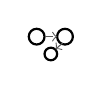
\begin{tikzpicture}[baseline]
            \draw[thick] (0.12, 0.32) circle (0.10);
            \draw[thick] (0.48, 0.32) circle (0.10);
            \draw[thick] (0.30, 0.10) circle (0.08);
            \draw[->, thin, gray!70!black, dashed]
                (0.22, 0.32) -- (0.38, 0.32);
            \draw[->, thin, gray!70!black, dashed]
                (0.45, 0.24) -- (0.36, 0.16);
        \end{tikzpicture}
    };

    \node[stage, right=of s4] (s5) {%
        \textbf{5}\\[-2pt]
        \scriptsize Emission\\[2pt]
        
\begin{tikzpicture}[baseline]
            \draw (0.05, 0) rectangle (0.55, 0.45);
            \foreach \y in {0.10, 0.20, 0.30, 0.38} {
                \draw[gray!60, very thin] (0.10, \y) -- (0.50, \y);
            }
        \end{tikzpicture}
    };

    % =========================================================
    % Pfeile
    % =========================================================
    \draw[flow] (s1) -- (s2);
    \draw[flow] (s2) -- (s3);
    \draw[flow] (s4) -- (s5);

    % =========================================================
    % Umbruch-Pfeil von s3 zu s4
    % WICHTIG: Mittelpunkt zuerst als eigene Coordinate ablegen,
    %          dann |- darauf anwenden.
    % =========================================================
    \coordinate (rowmid) at ($(s1.south)!0.5!(s4.north)$);
    \coordinate (w1) at ([xshift=0.4cm]s3.east);
    \coordinate (w2) at (w1 |- rowmid);
    \coordinate (w3) at (w2 -| s4);
    \draw[flow] (s3.east) -- (w1) -- (w2) -- (w3) -- (s4.north);

    % =========================================================
    % Labels OBERHALB der Pfeile
    % =========================================================
    \node[flowlabel, anchor=south]
        at ([yshift=2pt]$(s1.north east)!0.5!(s2.north west)$)
        {Höhen $a_i$};
    \node[flowlabel, anchor=south]
        at ([yshift=2pt]$(s2.north east)!0.5!(s3.north west)$)
        {Segmente};

    % Wrap-Label im Zwischenraum
    \node[flowlabel]
        at ($(w2)!0.5!(w3)$)
        {Konturringe};

    % Reihe 2
    \node[flowlabel, anchor=south]
        at ([yshift=2pt]$(s4.north east)!0.5!(s5.north west)$)
        {geordnete Ringe};

    % =========================================================
    % Eingabe und Ausgabe
    % =========================================================
    \draw[flow] ([xshift=-0.7cm]s1.west) -- (s1.west);
    \node[iolabel, anchor=east] at ([xshift=-0.75cm]s1.west)
        {\gls{mesh}};

    \draw[flow] (s5.east) -- ([xshift=0.7cm]s5.east);
    \node[iolabel, anchor=west] at ([xshift=0.75cm]s5.east)
        {Schicht-\\datensatz};

\end{tikzpicture}